\chapter{From 2D to 3D modeling}

\begin{quotation}
    \noindent
    \textsf{Till now, we have seen how Deep Learning can be used for solving Computer Vision tasks, and for tackling advanced tasks too (generative models, Human Pose Estimation, Human Action recognition). Anyway, another field in which the Deep learning approach can be used is the \textsf{computer graphics}. In this chapter we will present a couple of applications of this type. We will present the main aspects about \textit{3D data representation}, finally just to mention we will talk about \textit{Deep learning for Animation}. \\
    Note that we will introduce 3D data since they are of paramount importance in a lot of fields: computer graphics, robotics, additive manifacturing and so on.
    }
\end{quotation}

\section{Deep Learning for Computer Graphics}
One of the most important aspects in Machine learning is the \textbf{Task}. Formally a Task $T=\{\mathcal{Y},f\}$ is defined as learning a \textbf{mapping function} $f$ between an input space $\mathcal{X}$ and an output space $\mathcal{Y}$. In \textbf{Computer graphics} there are a certain number of tasks, each one involving different input and output spaces. In \Cref{tab:problems} there is a (non-exhaustive) list of possible tasks. 

\begin{table}[h!]
    \centering
    \begin{tabular}{|l|l|l|}
    \hline
    \textbf{Problem} & \textbf{Input $\to$ Output} & \textbf{Input $\to$ Output} \\ \hline
    Shape classification & 3D model $\to$ Label & $\mathbb{R}^{3d} \to \mathbb{R}^k$ \\ \hline
    Denoising, smoothing & Image $\to$ Image & $\mathbb{R}^{m \times m} \to \mathbb{R}^{m \times m}$ \\ \hline
    Inverse graphics & Photo $\to$ 3D model & $\mathbb{R}^{m \times m} \to \mathbb{R}^{3d}$ \\
    &Photo $\to$ Rendering &  $\mathbb{R}^{m \times m} \to \mathbb{R}^{m \times m}$ \\ \hline
    Animation & 3D model + time $\to$ 3D model & $\mathbb{R}^{3d \times t} \to \mathbb{R}^{3d}$ \\ \hline
    Generative models & Latent space $\to$ 3D model & $\mathbb{R}^k \to \mathbb{R}^{3d}$ \\ \hline
    \end{tabular}
    \caption{Some computer graphics tasks}
    \label{tab:problems}
\end{table}

In this chapter, we are going to treat the \textbf{inverse graphics} problems, that is how can we retrieve from a foto a \textbf{3D model} for the object/objects which are contained in it? Or, how can we retrieve several 2D images containing reflectance and shading?

\subsection{Neural Rendering}
How we will see later, in computer graphics and 3D animation field, there is an entire pipeline made up of a certain amount of modules by which some tasks can be performed. However, some of them can be replaced with Deep learning models such as \textit{neural networks}. In such a case we are talking about \textbf{Neural Rendering} whose ultimate goal is to obtain a \underline{more realistic} and \underline{less time consuming} rendering.\\
Many times the neural part is combined with Computer graphics (CG) components which can be differentiable or not. In the case they are \textbf{differentiable}, the entire architecture can be trained end to end by using forward and back-propagation, then the CG modules are embedded in the training process. The modified pipeline with the introduction of neural modules is shown in the following: 

\begin{figure*}[h]
    \centering
    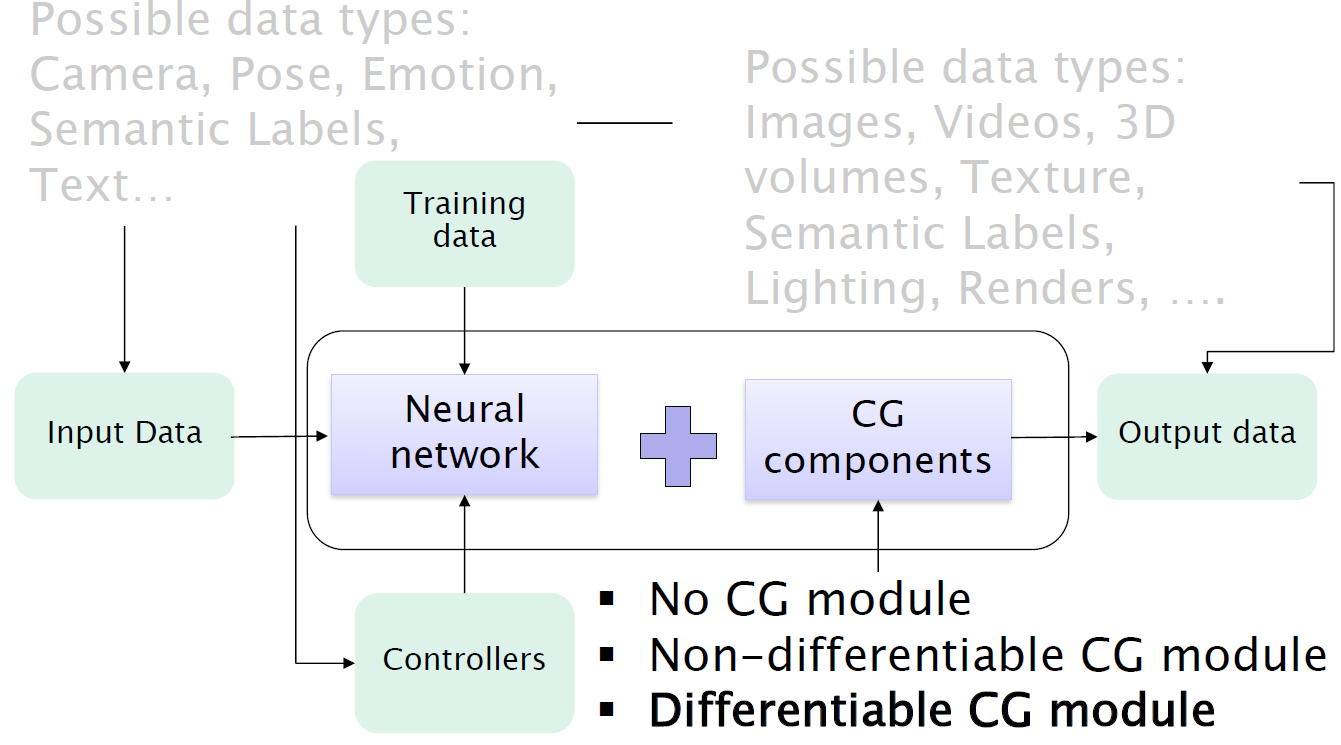
\includegraphics[scale=0.5]{img/NeuralRendering.png}
    \caption{Neural Rendering pipeline}
    \label{img:NeuralRendering}
\end{figure*}

Possible applications of neural rendering are \textit{denoising} a 'low-fi' image into an high resolution one, and \textbf{image decomposition} which is treated in the following subsection.

\subsection{Image to Rendering}

\subsubsection{Intrinsic image decomposition}
The human visual system has the ability to \textbf{decompose} entangled factors from the visual world into \textbf{simpler} underlying factors. The classical problem one wants to solve as CG task is the \textbf{decomposition} of \textit{reflectance} (albedo) and \textit{illumination} (shading) starting from an image. Unfortunately, such a problem is \textit{ill-posed} and \textit{under-constrained}. For this reason, some priors are needed to solve it properly. Just to provide an example in the work \citetitle{Zhou2015} \cite{Zhou2015}  (\citeauthor{Zhou2015}, \citeyear{Zhou2015}) \textbf{relative reflectance}\footnote{
    It is remarkable that humans are very good in estimating the difference in illumination between two pixels, rather than the absolute illumination.
} between pairs of pixels is estimated using human annotations in the Intrinsic Images in the \textit{Wild} dataset. Results are shown in \Cref{img:Zhou}.

\begin{figure}
    \centering
    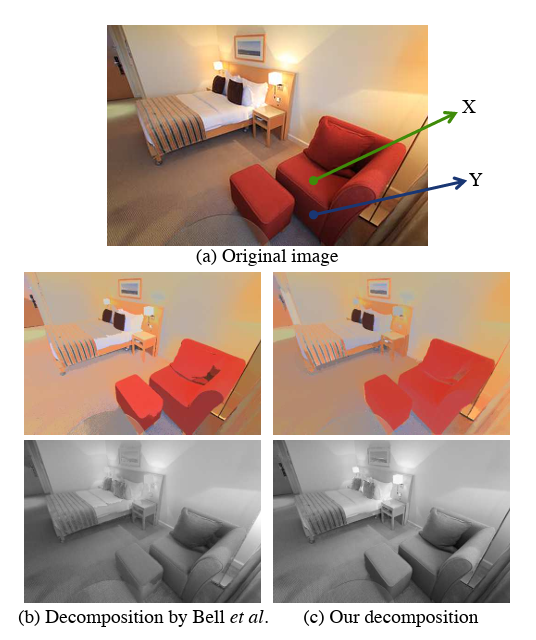
\includegraphics[scale=0.7]{img/Zhou.png}
    \caption{\textbf{Intrinsic image decomposition} here it is remarkable the fact that the reflectance for the sofa is uniform with respect to the state of art \textit{Bell et al.} model}
    \label{img:Zhou}
\end{figure}

\subsubsection{Image to Rendering with SfSNet}
A more advanced contribution to \textit{intrinsic image decomposition} is given in \citeauthor{SfSNet2018}, \cite{SfSNet2018} where the main objective is to decompose faces-in-the-wild into three components: (i)A \textbf{3D shape map} representing surface normals or depth. (ii) A \textbf{reflectance map} containing the albedo of the face. (iii) An \textbf{illumination map} (parameterized by spherical harmonics).

The overall deep learning architecture to address such tasks is given in the following. The main problem behind such a task is that there is no ground-truth for real images in terms of generated output layers (shading, normal, albedo). The solution is: train the architecture on synthetic data which are naturally labeled and then fine-tune the architecture with \textit{self-supervision}. The main problem to handle here is the gap between synthetic and real data. Fortunately, advances in generative techniques allows this gap to be closed. Very synthetically: 
\begin{itemize}
    \itemsep-0.3em
    \item A simple encoder-decoder architecture is trained on labeled \textit{synthetic data} to generate \textit{normal, albedo and lighting estimates}.
    \item The resulting network is used to obtain such a decomposition on given images; 
    \item The final SfSNet is trained mixing synthetic data (with ground truth) and real data (with authomatically generated labels); 
    \item A \textbf{photometric reconstruction loss}\footnote{ It is based on the image formation model
        $I=R \odot L(S)$ where $I$ is the reconstructed image, $R$ is the reflectance map, $L$ and $S$ are respectively the illuminance map and the shape (3D geometry, normal), while $\odot$ is the element-wise multiplication. 
    } is used in order to minimize the error between the original and reconstructed images (the ones are obtained by combining the three disentangled factors). This serves as \textbf{self-supervision} because the model uses the input image itself as the supervisory signal.
\end{itemize}
A problem that arises here is that Supervised learning can generalize poorly if real test data comes from a different distribution than the synthetic training data. To handle this issue we use supervised data when available and real world data with reconstruction loss in their absence.

\begin{figure*}[h]
    \centering
    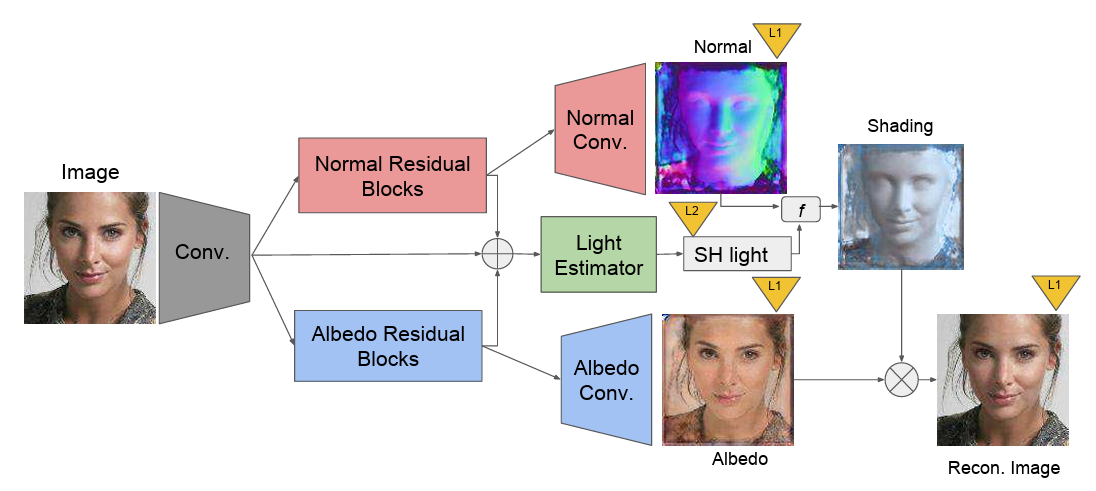
\includegraphics[scale=0.7]{img/SfSnet.png}
    \caption{SfSNet architecture [SfSNet consists of a novel decomposition architecture that uses residual blocks to produce normal and albedo features. They are further utilized along with image features to estimate lighting, inspired by a physical rendering model. f combines normal and lighting to produce shading. (Best viewed in color)]}    
\end{figure*}

\subsection{Image to 3D model}
Another inverse graphics problem listed in \Cref{tab:problems} is the task of obtaining the 3-dimensional shape from one or multiple views of a certain object. Also this problem is ill-posed since it suffers of \textit{self-occlusion}. The main idea behind an architecture which performs such a type of inverse graphics is the one presented in \Cref{fig:imgTo3D}

\begin{figure}
    \centering
    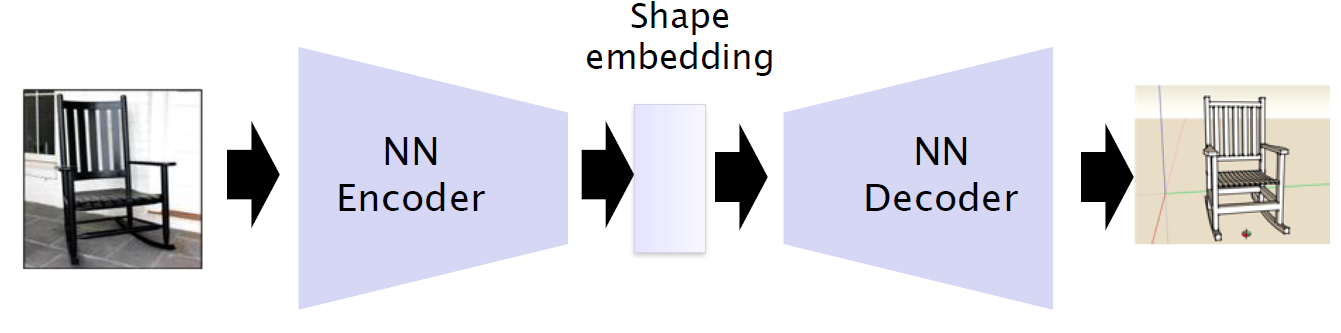
\includegraphics[scale=0.5]{img/img23D.png}
    \caption{Image to 3D model general architecture}
    \label{fig:imgTo3D}
\end{figure}
In this framework there is an important issue to solve: how can I represent 3D data? What is an \textbf{effective representation} for it.


\section{3D data representation}
3D data are very useful for computer vision tasks, they provide \textbf{rich information} about the full geometry of \textit{objects} and \textit{scenes}.
\begin{figure}[h]
    \centering
    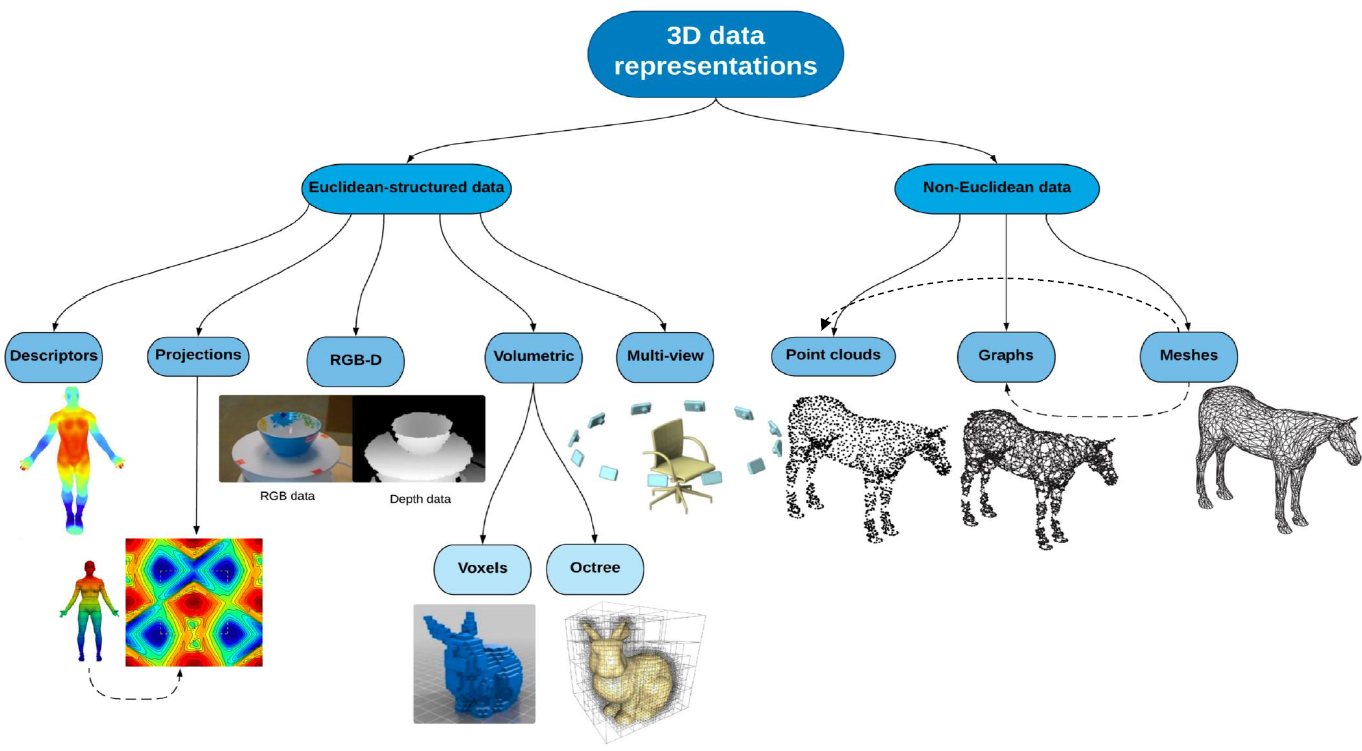
\includegraphics[scale=0.5]{img/3Drep.png}
    \caption{3D representation taxonomy}
    \label{fig:3D_taxonomy}
\end{figure}

The increasing advances in both computation and data availability make them more and more used. At a certain extent, according to their representation tailored architectures must be considered. In \Cref{fig:3D_taxonomy} there is a taxonomy for the principal 3D data representations. A more detailed description of the topics mentioned in the present paragraph can be found in \citeauthor{ahmed2018survey}, \cite{ahmed2018survey}. 3D-representations are split in two big categories:
\begin{itemize}
    \item \textsf{3D Euclidean Data}. They have an underlying \textbf{grid structure}, they are globally parametrized and use a common system of coordinates. Such interesting properties make the task of adapting the existing \textit{2D-architecture} quite straightforward; they are suitable to describe \textbf{mostly rigid object} where the deformation are minimal;
    \item \textsf{3D Non-Euclidean Data}. They have NOT a grid structure (we are talking about meshes,graphs and point clouds), this makes the 2D-architectures adaptation a challenging task. Such a type of 3D representation is useful for describing non-rigid objects (see human body) for several tasks (such as segmentation).
\end{itemize}

\subsection{Euclidian representations}
\subsubsection{Descriptors}
Given the 3D input shape they extract shallow features in order to feed different Deep Learning models with a simplified description of the tridimensional shape. The role of the neural network here is to learn from such simplified shapes more complex features. Just to mention \textbf{object descriptors} can be obtained by using object's \textit{geometry, topology, surface} or any other characteristic which can provide a signature for that object. \\
A famous example is SMPL which is a parametric human shape model which uses \textit{strong priors} on the human anatomy. By using 72 parameters it controls jointly shapes and pose. A nice feature is that SMPL is a \textbf{fully differentiable model}.

\subsubsection{3D data projections}
The main feature here is the projection of 3D data into a 2D space which could include the  \textbf{key properties} of that object/scene in 3D. Multiple types of projections  have been proposed in the literature. The most common is the mapping from the tridimensional into \textit{spherical} or \textit{cylindrical domain}. Deep  learning models for 2D processing are used in order to learn the new projected representation.
\subsubsection{RGB-D data}
The increasing popularity of RGB-D sensor makes the use of RGB-D images more and more used as a technique to address the problemn of representing 3D data. In particular such an approach provides insights about the 3D object by giving the \textbf{depth map} together with a 2D color information (RGB). The number of datasets with RGB-D images is larger with respect to other 3D-representation datasets.\\
There are some architectures (see \citeauthor{eitel28multimodal}, \cite{eitel28multimodal}) which first encodes separetely the depth and color stream, then they are fused in a single-stream architecture fashion.

\subsubsection{Volumetric data}
This is a type of representation which exploits a \textbf{regular grid} in a tridimensional space. Here the \textbf{voxels} are used in order to explain how the object is distributed in the three-dimensions of a scene. Voxels are not an efficient representation of the 3D scene since it encodes both occupied and non-occupied space resulting in an unnecessary use of memory storage. Moreover, \textbf{the representation is sparse} what is lost is the \textit{smoothness} of the surfaces. A more efficient representation of the 3D elementary unit is the \textbf{octree} which is a hierarchical data structure which better exploits the presence of empty voxels. Substancially an octree provides us with the possibility of representing \textbf{varying size} voxels, at the same time, and for this reason, they allows the representation of \textit{fine-grained details} for a certain 3D object. It is remarkable the fact that here the 3D CNN are used.

\subsubsection{Multi-view data}
Multiple 2D images extracted from a 3D input shape can be useful to describe the geometry of either an object or a scene. In practice, different 2D images from different point of views are extracted in order to jointly optimize the function representing the whole 3D object itself. Each separate view can be elaborated by a different 2D CNN in order to extract the main features. Such embedding are then merged and passed to another 'final' CNN in order to make the final decision.

\textsf{It is remarkable that studying \textit{3D euclidean representations} plays a noticeable role the 3D ConvNet models (eg. C3D), and 3D GAN.\\ Finally we remind that using a multi-view approach ease the use of standard 2D technologies for processing 3D information, the cons of such an approach is the time employed for the computations. At the opposite, using a \textit{volumetric data} provides the possibility to extend directly 2D-CNN into 3D-CNN, but as a drawbacks they suffer from sparse representation, or they exploit complex data structures (ie. octree)}. 

\begin{figure}
    \centering
    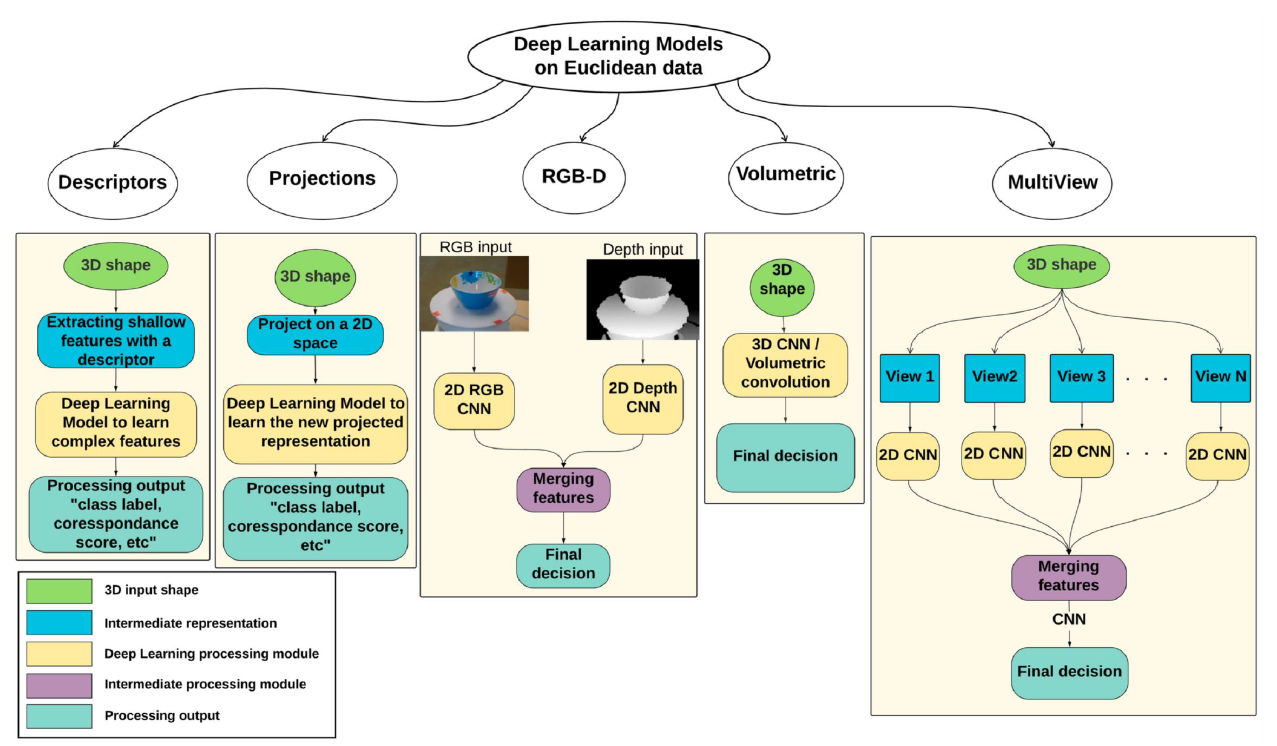
\includegraphics[scale=0.65]{img/EuclideanSummary.png}
    \caption{3D-Euclidean representations summary}
\end{figure}

\subsection{Non-Euclidean representations}
 
\subsubsection{3D-point clouds}
A \textbf{point cloud} can be seen as a set of \textbf{3D unstructured} points that \textit{approximate} the geometry of a 3D object. They can be analyzed by using ad-hoc architecture such as \textbf{Point Net}. Another approach is splitting a point cloud into a set of \textit{small  euclidean subsets} in order to exploit, again, volumetric convolutions.
Such a type of data is challenging to analyze due to the absence of a structure which leads to ambiguity about the structure information.

\subsubsection{3D meshes and graphs}
A \textbf{3D-mesh} is one of the most popular way to represent 3D shapes in a non-euclidean fashion. Its structure consists of:
\begin{enumerate}
    \itemsep-0.3em
    \item A \textbf{set of polygons} called \underline{faces} described in term of a \textbf{set of vertices}; 
    \item A \textbf{connectivity list} which describes how these vertices are organized and connected each other.
\end{enumerate}
How you can imagine the transformation of a mesh into a graph is straightforward, since the nodes correspond to the vertices of the polygons, the connectivity list is nothing but a list of edges between such nodes. There are tailored architectures which exploiting the \textit{graph laplacian} eigen-decomposition define a \textbf{convolution-like} operation on graphs or meshes converted into graphs.

\begin{figure}
    \centering
    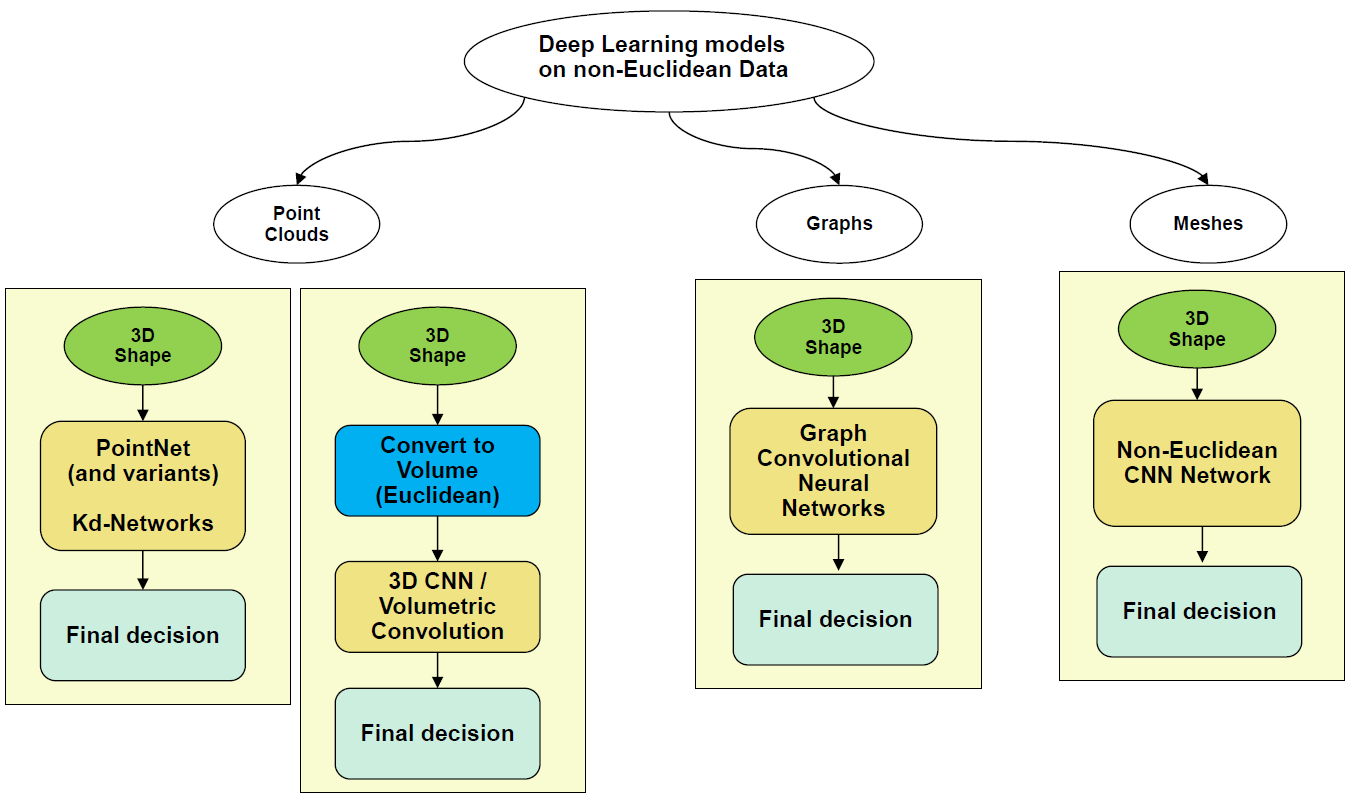
\includegraphics[scale=0.6]{img/NonEuclideanSummary.png}
    \caption{Non-Euclidean 3D representations Summary}
\end{figure}

\section{PointNet Classification Network}
The objective here is the introduction of an \textit{ad-hoc} architecture for \textbf{point clouds classification}. Since a point cloud is an \underline{unstructured} representation has some features which any tailored architecture must address:
\begin{itemize}
    \itemsep-0.3em
    \item \textsf{Permutation (order) invariance} A point clouds of $N$ points with $D$ coordinates can have $N!$ permutations, the output of the network must be the same independently from the points permutation.
    \item  \textsf{Geometric transformation invariance} The learned mapping must be invariant to \textbf{rotations} and \textbf{translations}.
    \item \textsf{Interactions among points} Points which are close each other form a \textbf{meaningful subset}, the representation which is learned by the architecture has to capture such local structures. This is fundamental for some tasks (eg. segmentation).
\end{itemize}

\subsection{Permutation Invariance}
The \textbf{permutation invariance} property can be achieved by using some \textbf{symmetric functions} such that:
\begin{equation}
    f(x_1,x_2,...,x_n) \equiv f(x_{\pi_1}, x_{\pi_2}, ..., x_{\pi_n})
\end{equation}
where $\pi_1,\pi_2,...,\pi_n$ is an arbitrary permutation. Examples of symmetric functions are the sum and the product among $D$-dimensional points. For example:
\begin{equation*}
    f(x_1,...,x_n)=x_1+...+x_n
\end{equation*}
In this context we need a way to build a \textit{family of symmetric functions} by using neural networks. As an observation we note that:
\begin{equation}
    f(x_1, x_2,...,x_n)=\gamma \circ g(h(x_1),h(x_2),...,h(x_n)) 
\end{equation}
is symmetric if $g$ is symmetric for any $\gamma, h$. Empirically speaking, simple functions such \textit{multi-layer perceptrons (MLP)} (for $h$ and $\gamma$) and max-pooling for $g$ (which is symmetric) are effective.
\subsubsection{Vanilla PointNet}
This first observation provides us a way to build a \textit{Vanilla PointNet architecture} (the paper in which such an architecture was proposed is \citetitle{qi2017pointnet}, \citeauthor{qi2017pointnet}, \cite{qi2017pointnet}) where $h$ is nothing but a \textbf{cascade of MLP} (with shared weights) each one taking a $D$-dimenisional point; the output of such a network is filtered by a \textit{max-pooling function} $g$. The result of such a layer is filtered by using a MLP $\gamma$ which in turn results in a features vector.

\begin{figure}
    \centering
    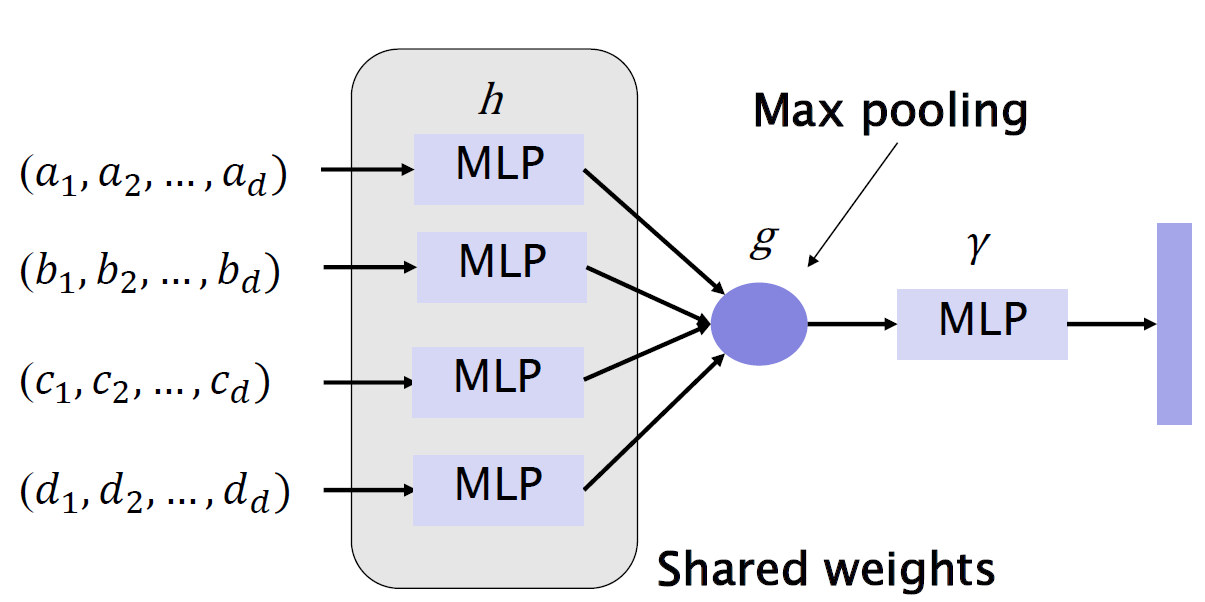
\includegraphics[scale=0.55]{img/VanillaPointNEt.png}
    \caption{PointNet (Vanilla Structure)}
\end{figure}

\subsection{Geometric invariance} 
The \textbf{Geometric invariance} is achieved by applying an input transformation to the point cloud in order to have the rotation invariance. In particular, the \textit{input transformation module} contains a \textbf{T-Net} (a spatial transformer network) in order to regress an orthogonal transformation matrix $T$ with dimensions compatible with the input point cloud. During the inference phase, such a matrix is used to multiply the point cloud and align it according to $T$, this produces again feature vector which can be elaborated again.\\
In order to ensure that $T$ remains a valid (orthogonal transformation) a regularization term is added of the type: 
\begin{equation*}
    L_{reg}=\Vert I-AA^T \Vert_F^2
\end{equation*}
Minimizing the \textit{Frobenius Norm} ($\Vert\cdot\Vert_F^2$), we ensure that the matrix $T$ is close to be orthogonal.

\begin{figure}[h]
    \centering
    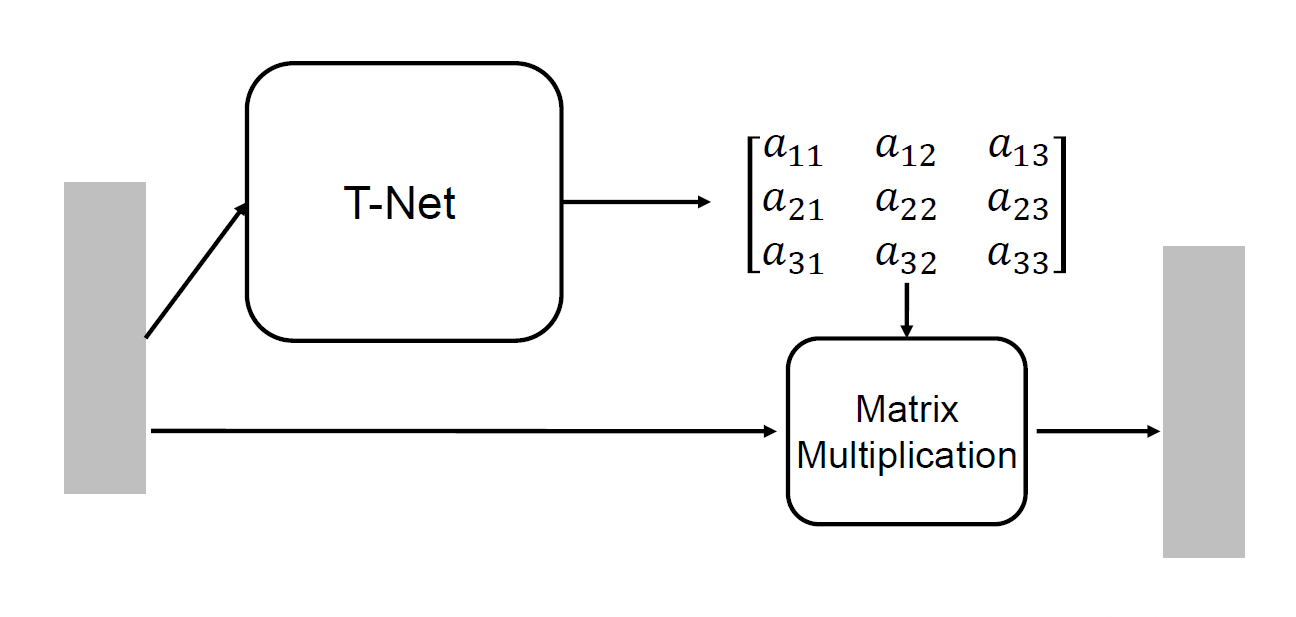
\includegraphics[scale=0.5]{img/PointNet_InputTrans.png}
    \caption{Input transformation module for PointNet}
\end{figure}

\subsection{PointNet complete structure}
The complete structure of PointNet is shown below, after input and feature transform with the module we have just explained, the max-pooling is applied in order to obtain a  \textit{global feature vector}, this ensure the \textbf{point interactions} since it represents a \textbf{composition of local embeddings} into a \textbf{global feature vector}. The same architecture is used for segmentation with the difference that a different branch of the model is exploited for the output.

\begin{figure}[h]
    \centering
    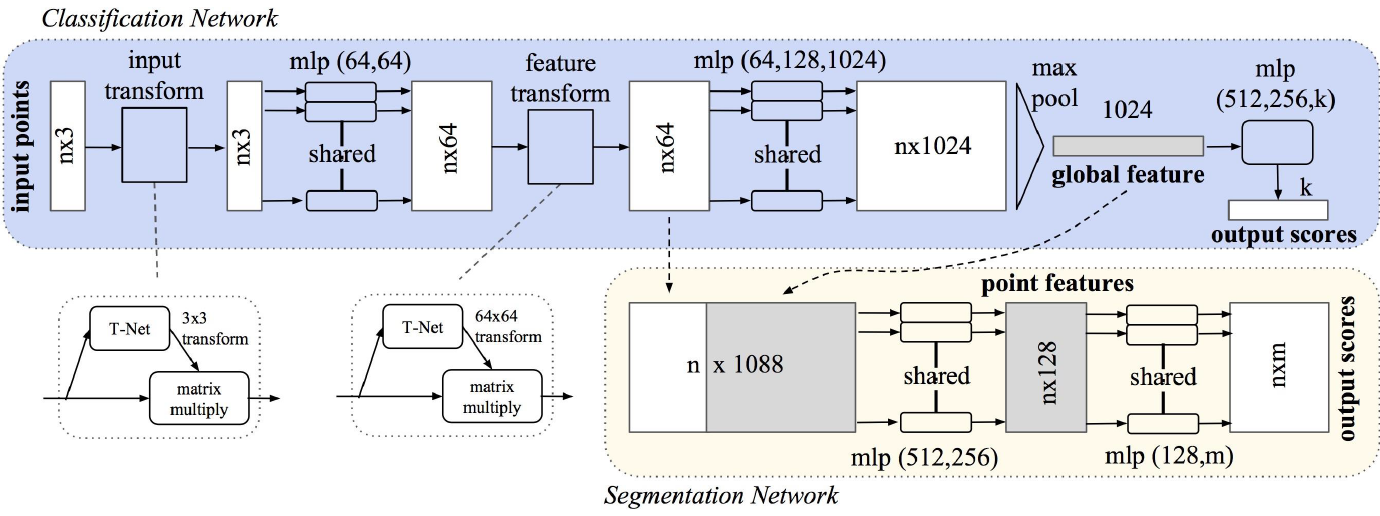
\includegraphics[scale=0.6]{img/PointNetFull.png}
    \caption{PointNet complete architecture}
\end{figure}

There is also an extension for PointNet which is \textit{PointNet++}, in this case the point cloud is not treated globally, there is an introduction of a hierachy in order to better learn local pattern (\textit{neighbourhood information}), in this field basic PointNet lacks since all points are treated independently. In other terms, the architecture first aggregate points into region extracting information from each of them, then such information are aggregated in order to extract higher level features.

\subsection{PointNet for point cloud synthesis}
PointNet was originally conceived for classication and segmentation tasks of 3D objects represented by using point clouds. The architecture can be also be adapted for another task which is the \textbf{point cloud synthesis}. In this context the \textbf{Earth Mover Distance (EMD)} plays a crucial role as a loss function. The input is a low-dimensional representation for example from an autoencoder or noise vector, the output is a set of 3D points related to the \textit{synthesized point cloud}. A neural network is used to map the latent representation to the 3D point cloud. 

\subsubsection{Earth Mover Distance (EMD)}
The \textbf{Earth Mover Distance} is a metric used to measure the similarity \textit{two point clouds}. It computes the \textbf{minimum cost of transforming one set of point into another}. 
\begin{definition}[Earth Mover distance]
    Given two point clouds $P$ and $Q$ containing $N$ points each, the EMD is defined as: 
    \begin{equation}
        L_{EMD}(P,Q)=\min_{\phi :P\to{Q}}{\sum_{p\in{P}} \Vert p-\phi(p)} \Vert
    \end{equation}
    where $\phi:{P}\to{Q}$ is a bijective mapping between the two point clouds and the norm is the distance between a point P and its mapping into a point of $Q$. This is nothing but finding the \textbf{optimal point to point correspondence}.
\end{definition}
\noindent
Datasets as \textsc{ShapeNet} are usually used as training.

\section{LIDAR processing and PointSeg}
\textbf{LIDAR} (Light Detection and Ranging) point clouds are a data format used for many applications in which there is the necessity to have outdoor point clouds which are \textbf{very large} and \textbf{very sparse}. Different architectures than PointNet are often needed to process them. LIDAR point clouds are generated by LIDAR sensors which \textbf{measure distances} by emitting laser pulses and recording the reflected signals. Here we provide a breakdown for the main features of such point clouds: 
\begin{enumerate}
    \itemsep-0.3em
    \item Each point in LIDAR point cloud is a 3D point (with $x,y,z$ coordinates).
    \item Many sensors also capture the intensity of the returned laser pulse;
    \item As point clouds they are unstructured representation of the 3D scene; 
\end{enumerate}

\subsection{Spherical Projection and LIDAR point clouds}
\textbf{Spherical projections} can be used in order to convert the LIDAR point cloud into a 2D image. In particular the steps are: 
\begin{itemize}
    \itemsep-0.3em
    \item Projecting the point cloud onto a sphere  by computing the spherical components ($\theta$ azimuth angle (horizontal axis), $\phi$ elevation angle (vertical axis) and $r$ distance); 
    \item Projecting such a sphere on a plan and optionally crop such an image to the field of view of the cameras. 
    \item Each projected point is associated with a pixel, moreover intensity and distance information can be encoded as additional image channels.
\end{itemize}

The \textbf{PointSeg} architecture (see \citetitle{pointseg} \cite{pointseg}) use such a 2D representation to adapting CNN architectures originally conceived for 2D image analysis. The input of the architecture is the 2D image obtained from the spherical projections of the LIDAR point cloud. This is very used in the field of autonomous driving for \textbf{real-time segmentation from point clouds}.

\begin{figure}
    \centering
    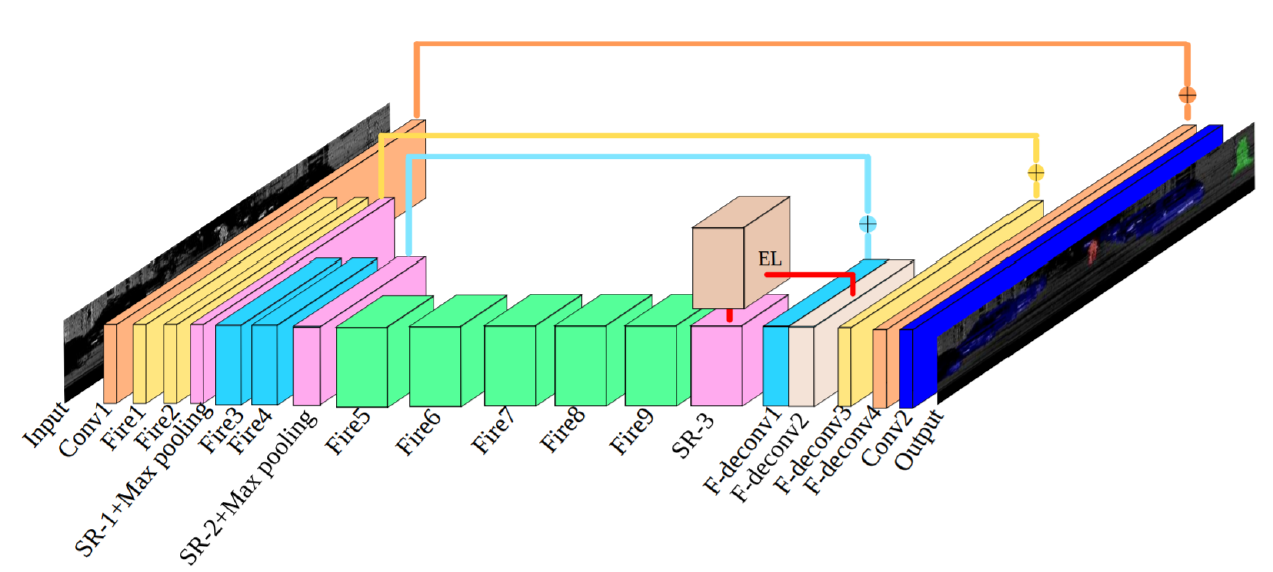
\includegraphics[scale=0.5]{img/PointSeg.png}
    \caption{PointSeg architecture}
\end{figure}

\section{Bird-Eye view}
\textbf{Bird-Eye View(BEV)} (from the top) is a popular representation in autonomous driving and robotics for converting \textbf{3D-point clouds or LIDAR} into a \textbf{2D top-down view} this consists in ignoring the third dimension $z$, while ($x,y$) coordinates are preserved. This 2D image-like structrure can be processed by pre-trained 2D CNN. In practice, the point cloud is transformed into a volumetric representation using voxels. When the representation is very sparse, the x,y information are coded into the 2D plane, while the statistics/point in the $z$ direction can be encoded as density in the BEV.\\
Usually we call: 
\begin{itemize}
    \item \textbf{Intensity} that returns from a point to the environment; 
    \item The \textbf{Density} refers to the number of LIDAR points into a specific voxel or grid cell in the BEV map. Higher density areas can be associated to \textit{solid object} with many points within a small region.
\end{itemize}

BEV images can be useful in general for:
\begin{enumerate}
    \itemsep-0.3em
    \item \textbf{Object Detection}:
    Intensity helps distinguish between reflective surfaces (e.g., vehicles) and non-reflective ones (e.g., vegetation).
    Density helps identify the structure and size of objects (e.g., a densely packed vehicle versus an empty road).
    \item \textbf{Semantic Segmentation}:
    Intensity helps with distinguishing materials (e.g., asphalt vs. grass), while density aids in segmenting solid objects or free space.
    \item \textbf{Obstacle Detection}:
Higher density areas correspond to objects, and higher intensity values may indicate reflective surfaces like vehicles or road signs.
\end{enumerate}

\section{3D Object Detection}
Just to mention Point based and volumetric based features can be used in order to train a model for \textbf{3D object detection}, the difference is mainly in the bounding boxes which are output in term of \textit{center coordinates}, \textit{dimensions} and \textit{orientation}. Roughly speaking each bounding box is a parallelepiped with given orientaition. \\The type of representation we use depends on the type of neural network will be used. Main 
steps are: (i) point cloud downsampling, (ii) feature extraction to convert 3D information to something suitable for a machine learning model, (iii) modeling and 3D object detection.

\section{Deep Learning for Animation}
An \textbf{animation} or \textbf{motion clip} $m\in\mathbb{R^{d\times{t}}}$ is defined by a temporal sequence of $t$ poses which can be expressed as a combination of the following features:
\begin{enumerate}
    \itemsep-0.3em
    \item \textbf{features} of a parametric model;
    \item positions of \textbf{J joints} in space; 
    \item as relative positions of the joints at time $t$ with respect to a root position;
    \item as a \textbf{graph} with $J$ nodes (joints). There are worksin which the this learned graphs show interactions not directly present in the reference skeleton.
\end{enumerate}

Possible related tasks are: 
\begin{itemize}
    \itemsep-0.3em
    \item \textsf{Motion Prediction/Synthesis} is a key task in autonomous driving and robotics, where the objective is to precict the future trajectories of dynamics objects (pedestrians, cyclists...) in a scene based on past motion and context information.
    \item \textsf{Interaction prediction/Synthesis} it is another crucial task for implementing autonomous vehicles and deal with forecasting how \textbf{multiple agents} interacts each other in a dynamic environment.
\end{itemize}

In the following there is a summarizing dcheme for the possible training techniques which are mainly \textit{Regression-based} or \textit{Reinforcement Learning based}.

\begin{figure}
    \centering
    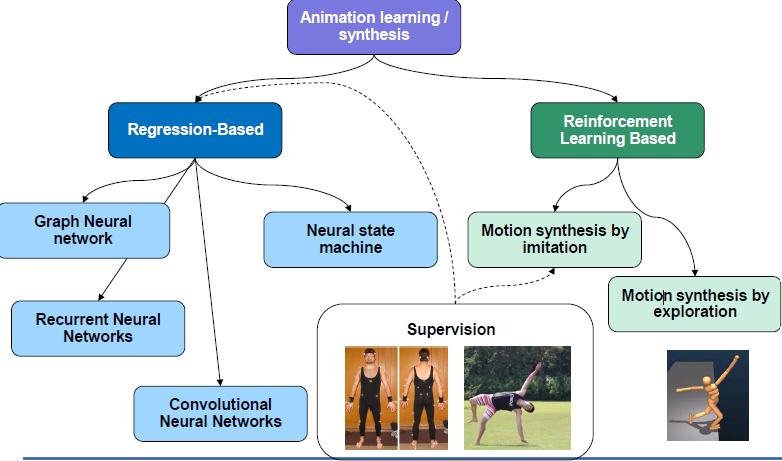
\includegraphics[scale=0.8]{img/MotionRecap.png}
    \caption{Training approaches for animation}
\end{figure}

\subsection{Motion encoding}
The paper by \citeauthor{holden2016deep}, \cite{holden2016deep} presents an innovative approach to create and edit 3D character animations using deep learning. The framework processes skeletal motion data. Dimensionality reduction techniques such as PCA are used in order to simplify motion data while retaining its essential features. A motion manifold is learnt by using an autoencoder architecture. If we sample some of their convolutional filters  we can note a strong temporal and inter-joint correlations. Moreover filters are sparse.

\begin{figure}
    \centering
    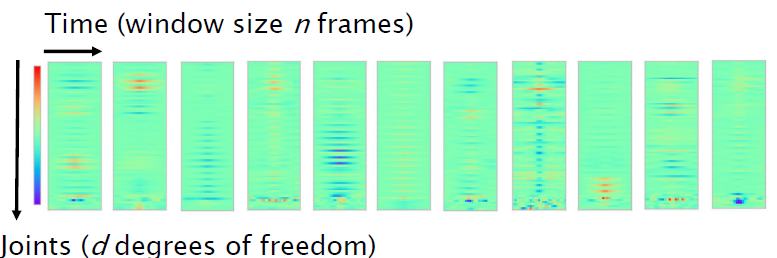
\includegraphics[scale=0.6]{img/MotionAutoenc.png}
    \caption{Convolutional filters from motion autoencoding}
\end{figure}

\subsection{Motion style transfer}
The paper \citetitle{aberman2020unpaired} by \citeauthor{aberman2020unpaired} enables the transfer of stylistic motion patterns from videos (or other motion sources) to \textbf{3D animated characters}, \underline{without requiring paired datasets}. For this reason such an architecture can be seen as a "Cycle GAN for animations". The method represent the motion in a \textbf{content-style disentangled latent space} where \textit{content} encodes the action (running, jumping...) while the \textit{style} encodes its specific features (speed, posture...).\\
The style is extracted from videos bypassing the extraction of motion data from the video itself. An \textbf{adversarial training} for Style transfer is used in order to ensure that the generated motion for the 3D character for a certain style is indistinguishable from the real motion sequences in that style.

\begin{figure}
    \centering
    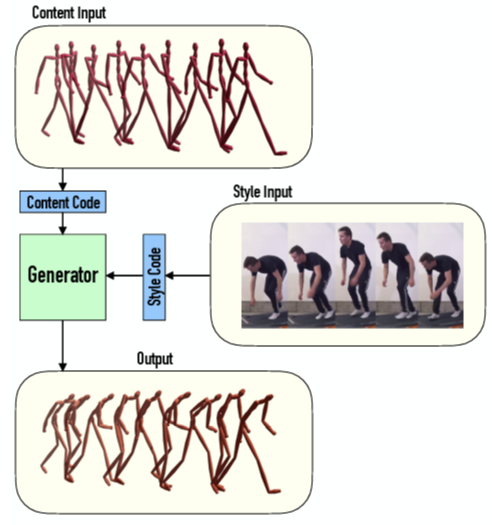
\includegraphics[scale=0.8]{img/MotionStyleTransfer.png}
    \caption{Motion style transfer main ideas}
\end{figure}

It is remarkable the content motion is represented by joint rotations by means of quaternions, while the style is inferred from joint positions. The overall architecture is presented below:
\begin{figure}
    \centering
    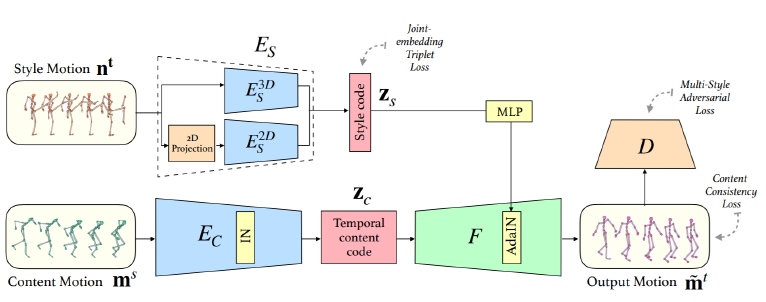
\includegraphics[scale=1]{img/MotionStyle_arch.png}
    \caption{Motion-style transfer architecture \textit{There is an encoder for the style $E_S$ which map the style motion into \textbf{style latent code}, while an encoder for content $E_C$ maps content motion data into a latent representation for content. This is provided together with the style latent code to the decoder that reconstruct the 3D motion sequience that \underline{incorporates the style} while preserving the original content. Instance normalization allows the disantanglement of content and style. A \textbf{content consistency loss} ensures identity mapping (same style) and that during the style transfer the content is preserved, while a discriminator uses a  \textbf{multistyle adversarial loss} in order to distinguish real from fake motions and improve the results from the decoder.}}
\end{figure}